\documentclass[a4paper, twoside, 10pt]{report}

\usepackage{color}
\usepackage{afterpage}
\usepackage{graphicx}
\usepackage{amsmath}
\usepackage[ddmmyyyy]{datetime}
\renewcommand{\dateseparator}{.}
\usepackage{setspace}
\usepackage{titlesec}
\usepackage{tikz}
\usetikzlibrary{calc}
\usepackage[margin=5cm]{geometry}
\usepackage{avant}

\usepackage[utf8]{inputenc}
\usepackage[english]{babel}
\usepackage{fancyhdr}
 
\pagestyle{fancy}
%\fancyhf{}
%\fancyhead[LE,RO]{\chapter}
%\fancyhead[RE,LO]{Guides and tutorials}
\fancyfoot[CE,CO]{\small{Johannes C. Mayer}}
\fancyfoot[LE,RO]{\thepage}

\titleformat{\chapter}
	{\normalfont\huge\bfseries}{\thechapter}{1em}{}
\titlespacing*{\chapter}{0pt}{3.5ex plus 1ex minus .2ex}{2.3ex plus .2ex}
\AtEndDocument{\cleardoublepage}

\title{Bachelor thesis booklet}
\author{Johannes C. Mayer}
\date{\today}

\newcommand\blankpage{\null\thispagestyle{empty}\addtocounter{page}{-1}\newpage}

\renewcommand{\familydefault}{\sfdefault}



\begin{document}

\begin{titlepage}

\begin{tikzpicture}[remember picture,overlay]
\node[inner sep=0pt] (background) at (current page.center) {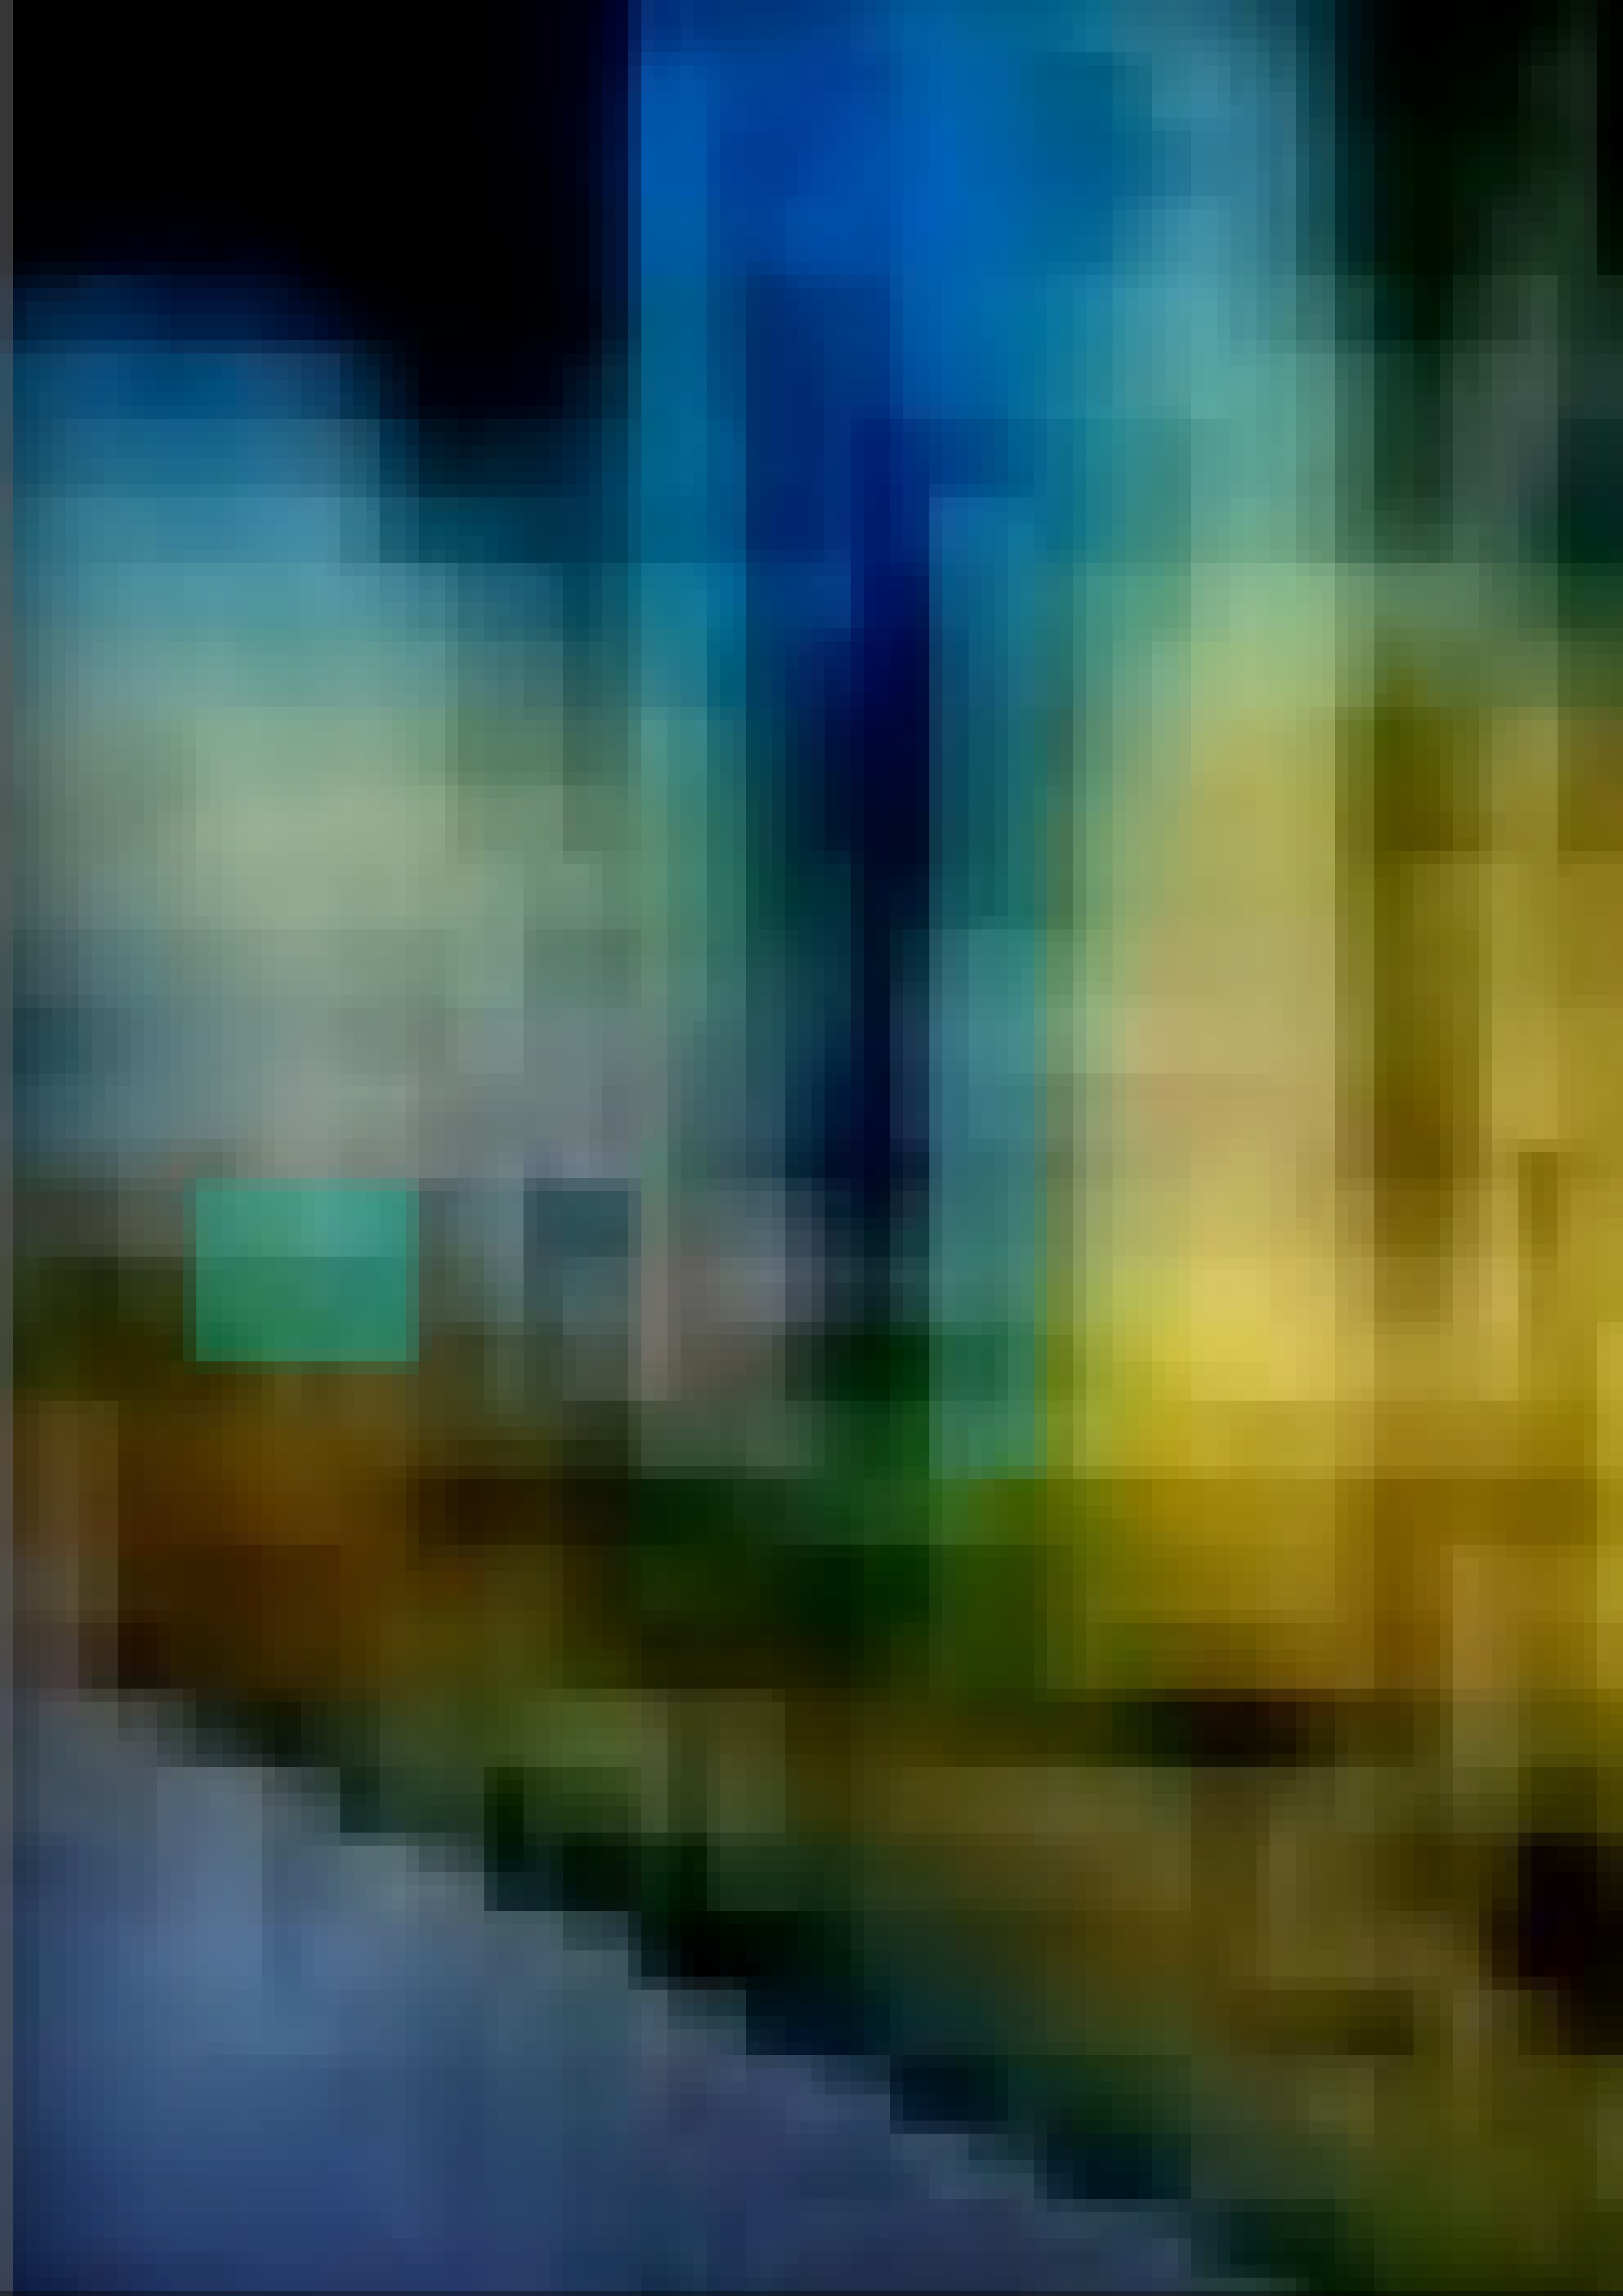
\includegraphics[width=\paperwidth]{Images/FrontCover.png}};
\draw ($(current page.south)+(0,5)$) node [fill=black,fill opacity=0.6,text opacity=1,inner sep=1cm]{\color{white}\Huge\centering\bfseries\sffamily\parbox[c][][t]{0.7\paperwidth}
{Shrouded Mirror\\[0pt]
{\Large Application of Neural Networks in interactive environments}\\[0pt]
{\Large Johannes C. Mayer}}};
\end{tikzpicture}
\end{titlepage}

\blankpage
\thispagestyle{plain}
\pagenumbering{Roman}

\begin{center}
\begin{spacing}{1.5}
{\Large
Bachelor thesis booklet in \\ the studies of GAME DESIGN \\
\vspace*{\fill}
The work constitutes a technical design work piece \\
\vspace*{\fill}
{\huge Shrouded Mirror} \\
Application of Neural Networks in interactive environments \\
\vspace*{\fill}
\textit{Submitted by} \\
Johannes C. Mayer, 553087 \\
\today \\
\vspace*{\fill}
\textit{First Examiner:} Prof. Thomas Bremer \\
\textit{Second Examiner:} Prof. Susanne Brandhorst \\
\vspace*{\fill}
Hochschule f\"ur Technik und Wirtschaft Berlin \\
Fachbereich Gestaltung und Kultur \\
}
\end{spacing}
\end{center}

\newpage

\tableofcontents
\cleardoublepage
\newpage
\pagenumbering{arabic}

\chapter{Introduction}
Shrouded mirror is an experimental experience, where the player sees the world through the eyes of a neural network. The player can move through the environment where different types of objects are placed. These objects behave differently and emit a unique audio signal, creating a distinctive sound scape.

\section{Expos\'e}
In my bachelor thesis I want to evaluate how neural networks can be used in an interactive context to visualize (an environments) state. For this three prototypes will be developed. The first two act as preparation for the last one which presents a sample application in an interactive context.

Neural networks have the ability to learn an abstract representations of the data being fed into it. This representation can then be used to generate new output. In this work a network is used, that is trained on data pairs, that consist of an Image and the corresponding coordinates, where the image was taken. {\color{red}TILL HERE REFACTOR STARTED} Combined with a set of scene coordinates to render an image that approximates very accurately what the actual camera would render when placed at the provided coordinates. This means that this technique can be used to create a virtual representation of an environment inside a game engine. 

Interesting possibilities open when integrating a GQN into an interactive environment. One example would be, that the player only sees the output of the GQN while the underlying “real” state of the environment is hidden from him. Now by manipulating the GQN we can influence how accurately its renderings are, in turn influencing what information is available to the player. One way this can be achieved is by deleting or adding new scene images to the representation network to encode into a new world model.

\subsubsection{Workflow}
The Project will be split up into three phases. Each phase will result in a prototype, that the following phase builds on.

\paragraph{I.  Implementation}
Determine which library to use. PyTorch, Chainer, Keras, Tensorflow are possible candidates. The first two might be prefered due to their ability to define computation graphs dynamically which would possibly allow the output size of the GQN to scale with screen size. With the selected library, a GQN is implemented into the target environment (most likely Unity).ii

\paragraph{II. Exploration}
The implementation of the GQN will now be investigated in regards to its manipulability and  constraintsivenes. The following questions will be answered:

Is it viable to inject additional parameters into the model, to enable more interesting behaviour?
What are the time constraints of applying a GQN into an interactive real time environment (training time, rendering time, updating worldmodel)?

Can a normal in game camera be overlayed with the output of the GQN?
Can objects be made to switch contexts of being displayed via GQN or camera dynamically?
Which interesting ways of interaction between player and the way the GQN behaves can be created, given other constraints?

\paragraph{III. Simple Application}
With the Gathered data on the limitations and possibilities a simple prototype application is conceptualized and developed. It demonstrates one or multiple scenarios in which the GQN can be applied to create or enhance an interactive environment.

\subsubsection{Work piece}
The following items will be produced during the Project:
\begin{itemize}
\item{Writing}
\item{Discussion of the Results form prototype II}
\item{Reflection on the project}
\item{Executable and source of prototype III}
\item{1 - 5 minutes video material, captured from interactions with prototype III}
\end{itemize}

\chapter{Background}

\section{Calculus}
\subsection{Univariate}
\subsection{Multivariate}
\subsection{Chain rule}
\subsection{What more?}
\section{Neural networks}
\subsection{Multilayer perceptron}
\subsection{Backpropagation}
\subsection{GQN Network}
\cite{gqn}

\chapter{Results}
\section{Training data generation}
\section{Model}
Model in python

\subsection{Structure}
In this work a network the architecture of GQN differs from the implementation used in the original paper. Here I use multilayer perceptron models for encoder and decoder without random latent variables. This circumvents the necessity of having to use methods like evidence lower bound estimation for optimization.

This however prevents the network from taking into account the inputs given during inference to the same extent as in the original experiments described in the paper. The only meaningful considerations of the inputs of the network were found to be the coloring of the sky, floor and walls (when the latter view have the same color). In the original implementation the network can correctly infer more properties like object position, rotation and texture.

Because interesting use cases where found, that do not depend on this property of the GQN network no more effort was put into recreating the ability of the network to model different scenes.

\subsection{Saving and loading}
\section{Data Preprocessing}
\section{Inter process communication}
UDP sending of player position to python

Motion JPEG over UDP socket 

\section{Rendering}
In Unity the stream is decoded and rendered using custom Cg shaders. These shaders merges the network output stream with objects in the environment that are tagged to be visible in the combined render.

Cull objects if hidden from camera pos in unity environment

\section{Player interaction}
\section{Prototypes}
Walking sim
Maze
Invisible Enemies

\chapter{Further work}
In this section possible further applications based on the found data is discussed.

\section{Other directions with current state}
\subsection{Multiplayer Game}
2 Players are task to take observations of an environment that is rendered within the unity engine in a limited time. These observations  are now used as training data for a GQN. After training both player have to fight each other in this environment using the rendered output of the GQN.

\subsection{Merge output of multiple models}
\subsection{Blending of internal network state}
Lerp some parameters to network to create effect.

\section{Expand GQN capability}
GQN hard so not very good implementation. Variational metods, random ratent variables. Therefore only MLP.

\subsection{Generative model for modeling environment}
\subsection{Implement original GQN}
\subsection{Implement environment time step prediction}
\section{Expanded GQN directions}

\chapter{Resources}
\section{Software}
\begin{itemize}
\item Unity3D
\item Git
\item Visual Studio
\item Python
\item PyCharm
\item Blender
\item Krita
\end{itemize}

\section{Python packages}
\begin{verbatim}
_tflow_select=2.1.0=gpu
absl-py=0.6.1=py36_0
astor=0.7.1=py36_0
blas=1.0=mkl
ca-certificates=2018.03.07=0
certifi=2018.10.15=py36_0
cudatoolkit=9.0=1
cudnn=7.1.4=cuda9.0_0
cycler=0.10.0=py36h009560c_0
freetype=2.9.1=ha9979f8_1
gast=0.2.0=py36_0
grpcio=1.12.1=py36h1a1b453_0
h5py=2.8.0=py36h3bdd7fb_2
hdf5=1.10.2=hac2f561_1
icc_rt=2017.0.4=h97af966_0
icu=58.2=ha66f8fd_1
intel-openmp=2019.0=118
jpeg=9b=hb83a4c4_2
keras-applications=1.0.6=py36_0
keras-preprocessing=1.0.5=py36_0
kiwisolver=1.0.1=py36h6538335_0
libpng=1.6.35=h2a8f88b_0
libprotobuf=3.6.1=h7bd577a_0
libtiff=4.0.9=h36446d0_2
markdown=3.0.1=py36_0
matplotlib=3.0.1=py36hc8f65d3_0
mkl=2019.0=118
mkl_fft=1.0.6=py36hdbbee80_0
mkl_random=1.0.1=py36h77b88f5_1
numpy=1.15.3=py36ha559c80_0
numpy-base=1.15.3=py36h8128ebf_0
olefile=0.46=py36_0
openssl=1.0.2p=hfa6e2cd_0
pandas=0.23.4=py36h830ac7b_0
pillow=5.3.0=py36hdc69c19_0
pip=10.0.1=py36_0
protobuf=3.6.1=py36h33f27b4_0
pyparsing=2.2.2=py36_0
pyqt=5.9.2=py36h6538335_2
python=3.6.7=h33f27b4_1
python-dateutil=2.7.5=py36_0
pytz=2018.7=py36_0
qt=5.9.6=vc14h1e9a669_2
scipy=1.1.0=py36h4f6bf74_1
setuptools=40.5.0=py36_0
sip=4.19.8=py36h6538335_0
six=1.11.0=py36_1
sqlite=3.25.2=hfa6e2cd_0
tensorboard=1.11.0=py36he025d50_0
tensorflow=1.11.0=gpu_py36h5dc63e2_0
tensorflow-base=1.11.0=gpu_py36h6e53903_0
tensorflow-gpu=1.11.0=h0d30ee6_0
termcolor=1.1.0=py36_1
tk=8.6.8=hfa6e2cd_0
tornado=5.1.1=py36hfa6e2cd_0
vc=14.1=h0510ff6_4
vs2015_runtime=14.15.26706=h3a45250_0
werkzeug=0.14.1=py36_0
wheel=0.32.2=py36_0
wincertstore=0.2=py36h7fe50ca_0
zlib=1.2.11=h8395fce_2
\end{verbatim}

\section{Unity packages}
\begin{itemize}
\item MK Toon Free (Toon shader) % & https://assetstore.unity.com/packages/vfx/shaders/mk-toon-free-68972 \\
\item Post Processing Stack % & https://assetstore.unity.com/packages/essentials/post-processing-stack-83912 \\
\item ml-agents % & https://github.com/Unity-Technologies/ml-agents \\
\item Universal Sound FX % & https://assetstore.unity.com/packages/audio/sound-fx/universal-sound-fx-17256 \\
\item Realistic Effects Pack % & https://assetstore.unity.com/packages/vfx/particles/spells/realistic-effects-pack-4-85675 \\
\item Standard Assets % & https://assetstore.unity.com/packages/essentials/asset-packs/standard-assets-32351 \\
\item Ultimate Game Music Collection % & https://assetstore.unity.com/packages/audio/music/orchestral/ultimate-game-music-collection-37351 \\
\item Resonance Audio SDK for Unity v1.2.1 % & https://github.com/resonance-audio/resonance-audio-unity-sdk/releases \\
\item UPFS: Ultimate FPS % & https://assetstore.unity.com/packages/templates/systems/ufps-ultimate-fps-2943 \\
\end{itemize}

\section{Textures}

\bibliographystyle{plain}
\bibliography{BachelorBooklet}

\listoffigures
\listoftables

\chapter*{Acknowledgments}
I would like to thank my professors and fellow students, who gave feedback that helped me to steer the project in the right direction.

\chapter*{Statement of Authorship}
I hereby declare that I am the sole author of this bachelor thesis and that I have not used any sources other than those listed in the bibliography- and resources section. I further declare that I have not submitted this thesis at any other institution in order to obtain a degree.
\begin{spacing}{4}
\noindent
(Place, Date)\dotfill \space (Signature)\dotfill
\end{spacing}

\newpage
\pagestyle{empty}
\centering
\vfill

\includegraphics[width=0.5\textwidth]{Images/logo_GD_black.jpg}
\vfill
\vspace*{-2cm}

\includegraphics[width=0.5\textwidth]{Images/logo_dehive.jpg}
\vfill

\includegraphics[width=0.5\textwidth]{Images/logo_htw.jpg}
\vfill

\newpage
\blankpage

\begin{tikzpicture}[remember picture,overlay]
\node[inner sep=0pt] (background) at (current page.center) {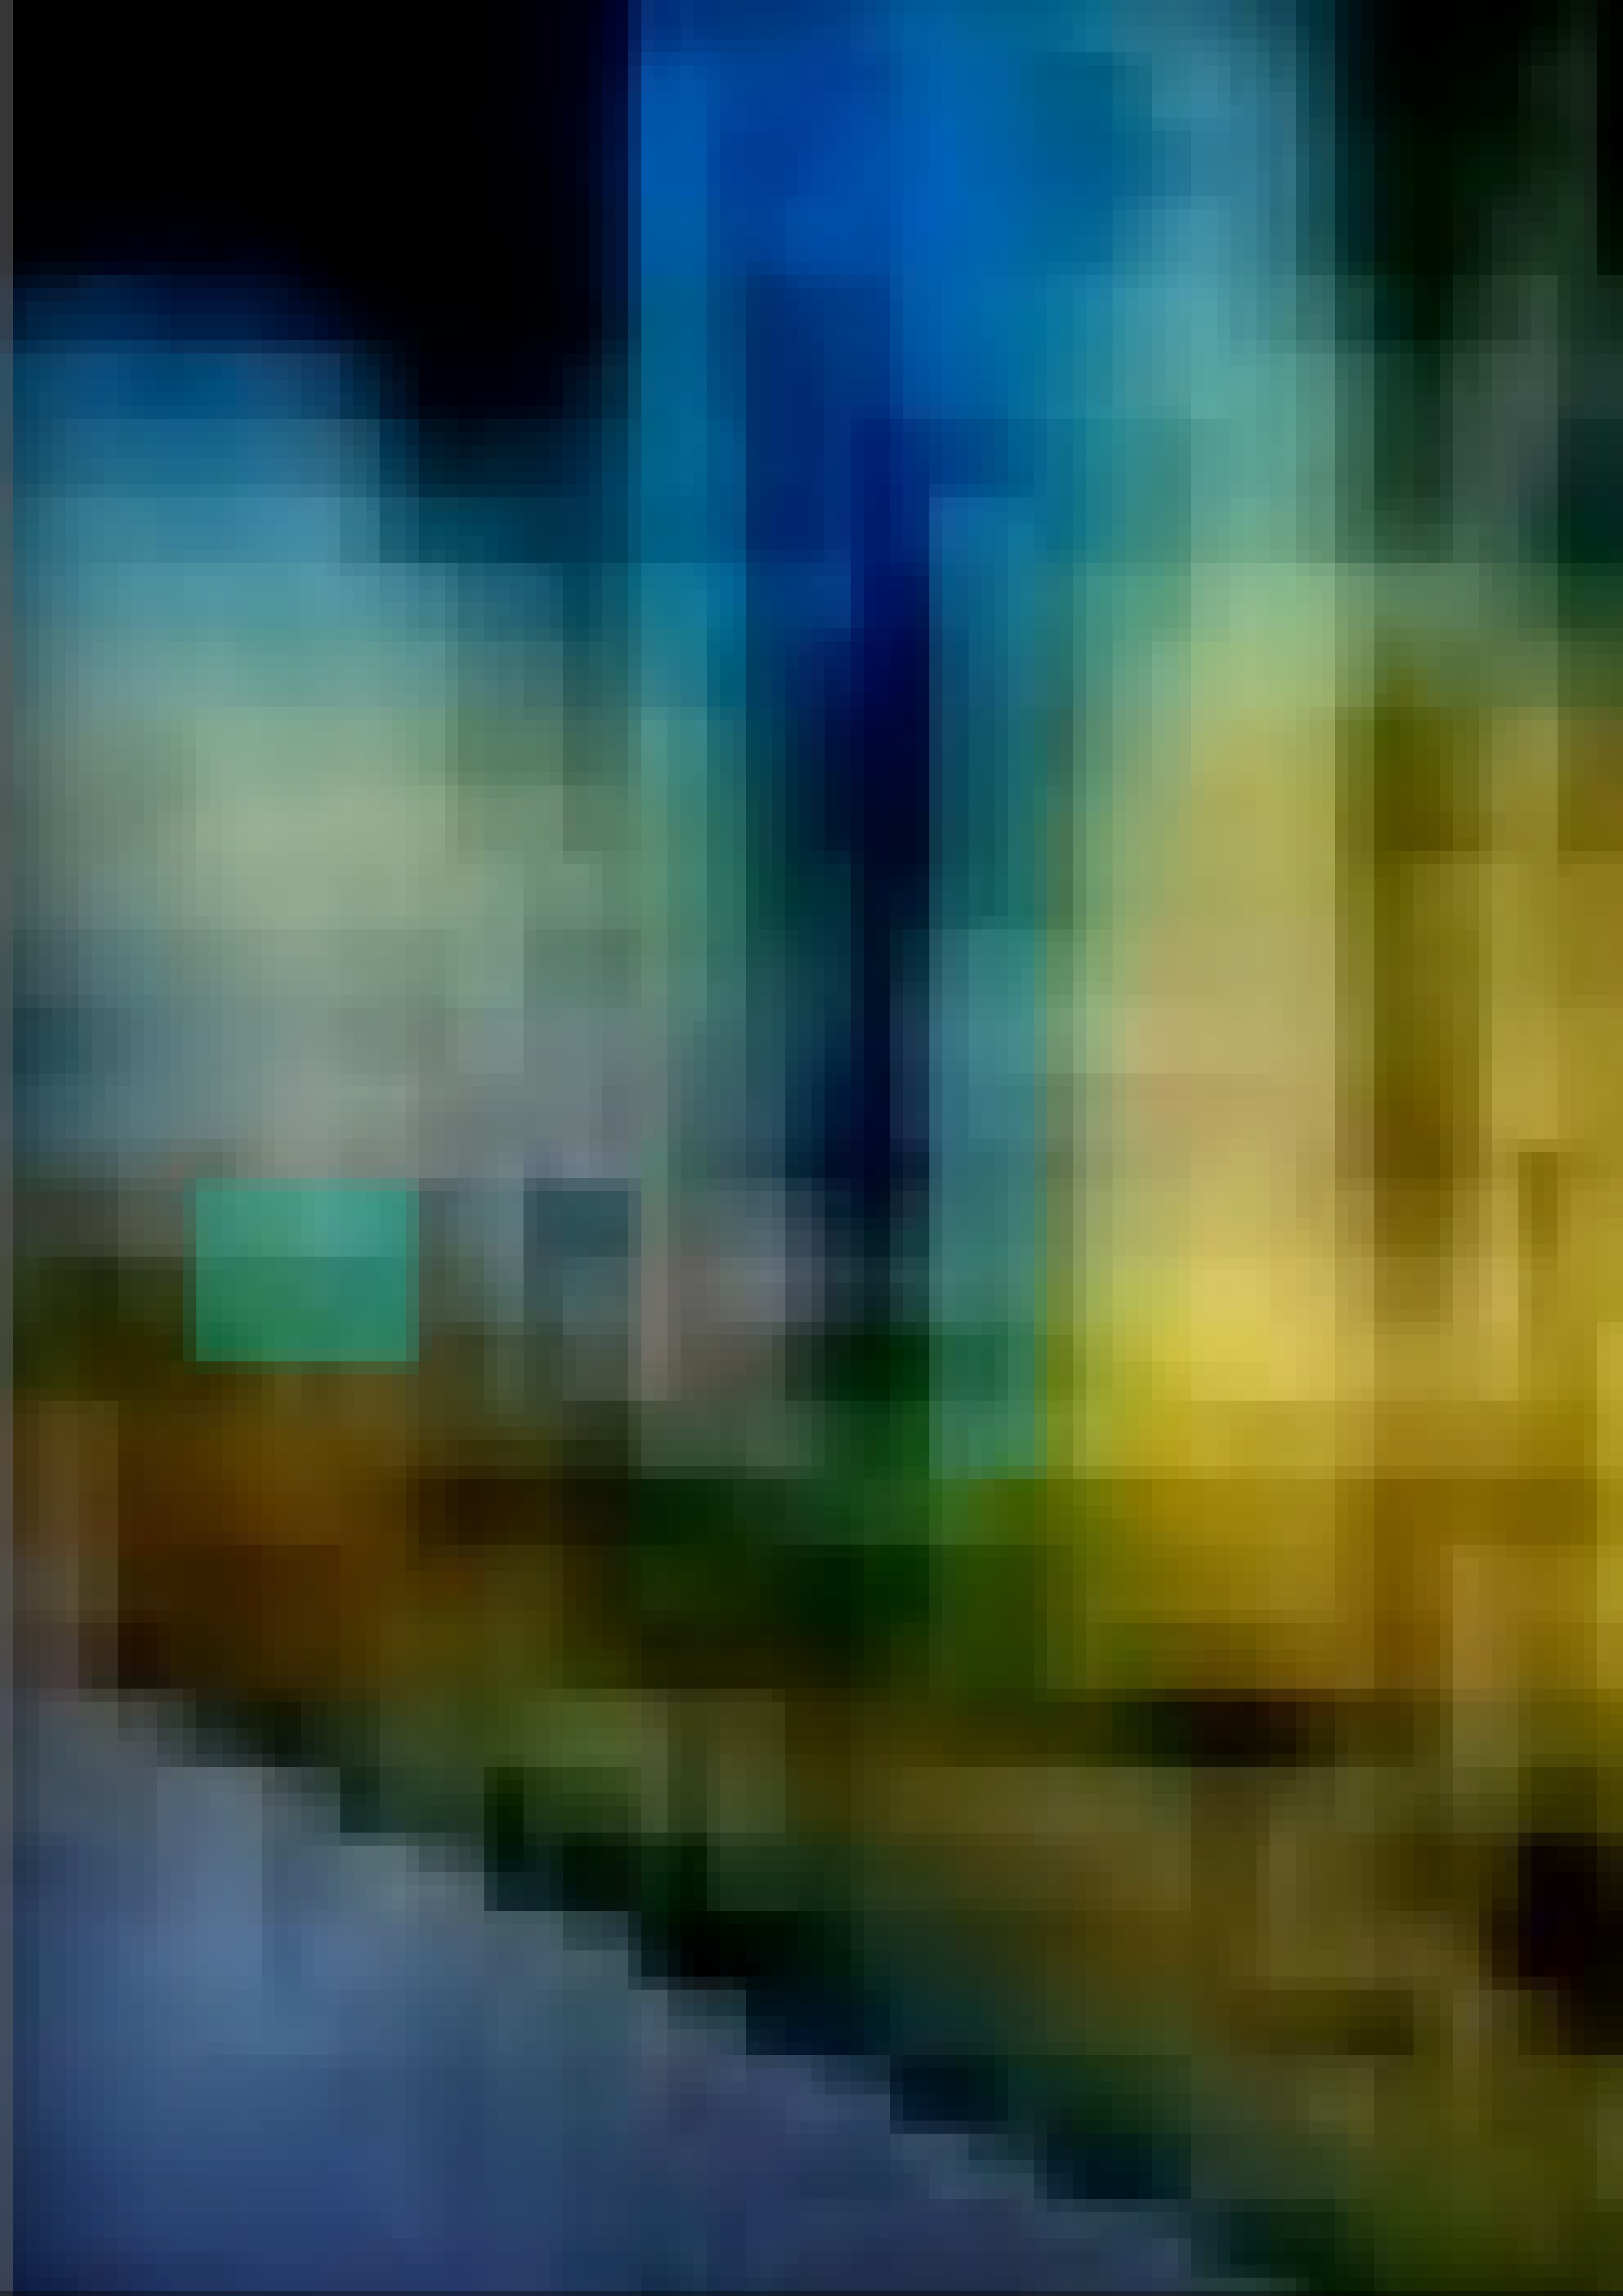
\includegraphics[width=\paperwidth]{Images/BackCover.png}};
\end{tikzpicture}

\end{document}